% ==============
% COJAC analysis
% ==============

\chapter{COJAC}

\section{Instrumentation}

\section{Maven}

COJAC utilise Maven \cite{maven} pour créer le JAR. Maven \cite{maven} est un outil d'automatisation pour gérer les dépendances et produire une application. Cet outil peut télécharger les dépendances, compiler le projet, exécuter les tests unitaires et d'intégration et déployer le projet. Maven et Graddle sont les deux outils les plus souvent utilisés pour gérer les projets Java. Toute la configuration se trouve dans le fichier \textit{pom.xml}.

\subsection{Debug}

Lorsqu'il y a un problème avec Maven, il y a plusieurs paramètres qui permettent d'obtenir plus d'informations. Cette section montre comment configurer ces paramètres sous IntelliJ et donne l'argument équivalent pour appeler Maven en ligne de commande.

\subtitle{Ouvrir la fenêtre Maven}

Toutes les configurations effectuées ci-dessous seront effectuées depuis la fenêtre Maven dans IntelliJ. Le bouton pour l'ouvrir se situe sous \textbf{View} $\rightarrow$ \textbf{Tool Windows} $\rightarrow$ \textbf{Maven} comme montré sur la figure \ref{fig:maven_open_window}.

\begin{minipage}{\linewidth}% to keep image and caption on one page
\makebox[\linewidth]{%        to center the image
    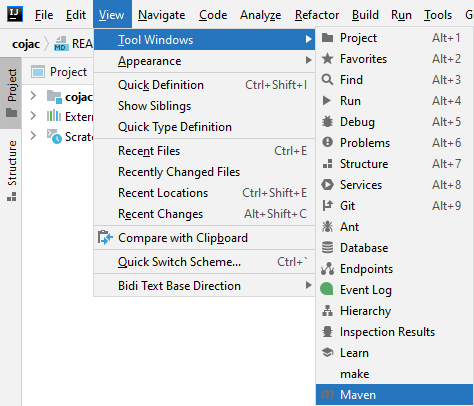
\includegraphics[width=.7\linewidth]{maven/open_maven_window.png}
}
\captionof{figure}{Bouton d'ouverture de la fenêtre Maven}
\label{fig:maven_open_window}
\end{minipage}

\subtitle{Fenêtre Maven}

La fenêtre Maven montre le contenu du projet avec les étapes du cycle de vie de la production de l'application comme le montre la figure \ref{fig:maven_window}. Le bouton encadré sur l'image permet d'ouvrir les paramètres de Maven qui seront utilisés plus tard. On peut également voir les plugins et les dépendances. Cette fenêtre permet aussi d'exécuter les étapes pour produire l'application. L'étape \textit{package} est suffisante pour générer le JAR.

\begin{minipage}{\linewidth}
\makebox[\linewidth]{
    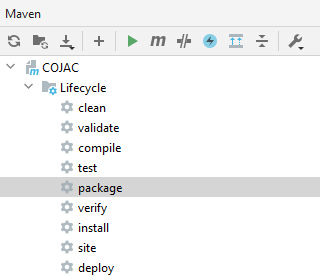
\includegraphics[width=.5\linewidth]{maven/maven_window_annotated.png}
}
\captionof{figure}{Fenêtre Maven}
\label{fig:maven_window}
\end{minipage}

Une option peut être ajoutée pour afficher les messages de debug. Cette option est plus souvent utilisée lors du développement de Maven ou d'un plugin Maven. Cependant, elle peut également être utile pour trouver la source d'un problème difficile. \todo{image}. L'option en ligne de commande équivalente se nomme \textit{-{}-debug}.